\documentclass[uplatex,dvipdfmx]{jsarticle}

\usepackage[uplatex,deluxe]{otf} % UTF
\usepackage[noalphabet]{pxchfon} % must be after otf package
\usepackage{stix2} %欧文＆数式フォント
\usepackage[fleqn,tbtags]{mathtools} % 数式関連 (w/ amsmath)
\usepackage{hira-stix} % ヒラギノフォント＆STIX2 フォント代替定義（Warning回避）
\usepackage{float}
\usepackage{multirow}


\begin{document}
\section{26班作業ログ}
報告者:[三芝空音]\\


報告日:[\today]\\


プロジェクト名:[単一のフルカラー LED と Arduino を用いた光無線通信による楽器間同期演奏システムの開発]\\


\section{人員ごとの作業時間統計}

人員ごとの作業時間の統計を表\ref{tab:time}に示す．
5週目では，主に基本設計および各機能の試作を中心に作業を行った．
特に，楽器音作成や同期システムの実装を担当したメンバーの作業時間が多くなっている．\\
6,7週目では，5週目と比較して作業時間の増加が見られるメンバーが多く，実装作業が本格化していることがわかる．
8週目では，楽器音が完成したので，全体のシステムの結合に移っている．
シリアル通信単体，webでの開始，停止テンポ変更，音再生単体は完成している．
9週目，10週目では結合と全体のテストを行い，システムとしての完成を目指し，各々作業を進めている．
\begin{table}[H]
  \centering
  \caption{人員ごとの作業時間統計}
  \label{tab:time}
  \renewcommand{\arraystretch}{1.2}
  \scalebox{0.68}{
    \begin{tabular}{|c|c|c|c|c|c|c|}
      \hline
        & 5週目 & 6,7週目 & 8週目 & 9週目 & 10週目& 11週目 \\ \hline
      三芝& 15 & 4 & 5 & 5 &8 & - \\\hline
      荘司& 13.5& 11 & 9 & 7 &8 & - \\\hline
      金枝& 3 & 18 & 7 & 7 & 7 & - \\\hline
      佐藤& 25 & 21 & 17 & 12 & 13 & - \\\hline
      飯塚& 12.5 & 23 & 12 & 6 &24 & - \\\hline
      恩田& 7 & 19 & 8 & 22 & 9 & - \\\hline
    \end{tabular}
  }
\end{table}



\section{WBSの要素ごとの作業時間の統計}
WBS要素ごとの作業時間の統計を表\ref{tab:WBStime}に示す．
5週目では，光通信機能および楽器音生成機能の実装に多くの時間を要した．
また，Webサイト機能やLEDマトリクス演出についても並行して作業を進めた．\\
6,7週目では，ヴァイオリン音およびパーカッション音など，楽器音作成に関する作業時間が大幅に増加した．
一方，設計フェーズの作業はほぼ完了し，実装に重点が移っていることがわかる\\
8週目では，楽器音作成の完成により，楽器音関連の時間が減少した．
現在は単体での動作確認とフルカラーLEDでの送受信に注力している．

9週目では，前回までに1楽器の状態で指揮者から演奏者までを繋げて演奏することができた．
今回の作業は，演奏する楽器を増やしても輪唱が成立するかの作業をした．

10週目では結合と評価指標のためのアンケートの作成，発表のためのスライド作成を行なった．
先週と比べ，演奏者が一定時間LED点滅を受け取らないと演奏番号をリセットする機能を追加した．
\begin{table}[H]
  \centering
  \caption{WBSの要素ごとの作業時間の統計}
  \label{tab:WBStime}
  \renewcommand{\arraystretch}{1.2}
  \scalebox{0.68}{
    \begin{tabular}{|c|c|c|c|c|c|c|}
      \hline
        & 5週目 & 6,7週目 & 8週目 & 9週目 & 10週目& 11週目 \\ \hline
      全体基本設計・詳細設計& 8.5 & 0 & - & - &- & - \\\hline
      楽器演奏基本設計& 1 & 0 & - & - &- & - \\\hline
      受光機能詳細設計& 3.5 & 7 & - & - &6 & - \\\hline
      ArduinoProcessing間通信詳細設計& 1 & 0 & - & - &- & - \\\hline
      LEDマトリクス& 6 & 1 & - & 3 &- & - \\\hline
      楽譜配列の作成& 1& 4 & - & 1 &- & - \\\hline
      機材調達& 2 & 0.5 & - & - &- & - \\\hline
      ピアノ音& 4 & 3 & 7 & - &- & - \\\hline
      フルート音& 3 & 2 & 1 & - &- & - \\\hline
      ヴァイオリン音& 2 & 13 & 5 & - &- & - \\\hline
      パーカッション音& 3& 11 & 1 & - &- & - \\\hline
      光信号発信& 7.5 & 5 & 4 & 1 &- & - \\\hline
      受光機能& 3 & 5 & 4 & 1 & 6 & - \\\hline
      webサイト & 3 & 3 & 5 & 6 &- & - \\\hline
      テンポ変更機能& 7.5 & 3 & 1 & - &- & - \\\hline
      シリアル通信& 7.5 & 3 & 8 & 2 &- & - \\\hline
      開始停止スイッチ& 3 & 2 & 4 & - &- & - \\\hline
      同期演奏システムの結合& - & - & - & 21 &12 & - \\\hline
      楽器音テスト& - & - & - & 21 &5 & - \\\hline
      開始停止スイッチテスト& - & - & - & 1 & 2 & - \\\hline
      テンポ変更スイッチテスト& - & - & - & 1 & 2 & - \\\hline
      Web通信テスト& - & - & - & 1 & 2 & - \\\hline
      光通信同期テスト& - & - & - & 1 & 2 & - \\\hline
      接続テスト& - & - & - & 1 & 2 & - \\\hline
      遅延テスト& - & - & - & 1 & 2 & - \\\hline
      演奏成立テスト& - & - & - & 1 & 2 & - \\\hline
    \end{tabular}
  }
\end{table}



\section{作業の進捗率: WBSとガントチャート}
本開発における作業分解構造WBSと管理番号を表\ref{WBS}に，現在のガントチャートを図\ref{fig:ガントチャート変更後}に示す．
楽器音単体の遅延テストは結合の方へ項目を移した．
\begin{table}[H]
\centering
   \caption{本開発におけるWBSと管理番号}
   \label{WBS}
\resizebox{\textwidth}{!}{ %
\begin{tabular}{|l|l|l|l|l|} \hline
   目的 &フェーズ & タスク&活動タスク&担当者 \\ \hline
\multirow{1}{*}{LEDの発光色による光同期システム}
& \multirow{1}{*}{100設計}
							 & \multirow{1}{*}{110基本設計} &111楽器演奏&2年\\\cline{4-5}
							 && &112Webサイト&金枝\\\cline{4-5}	
							&& &113LEDマトリクスデザイン&3年\\\cline{3-5}		
    							&&\multirow{1}{*}{120詳細設計}&121LED点滅機能&佐藤\\\cline{4-5}
							&& &122受光機能&飯塚\\\cline{4-5}
							&& &123演奏開始・停止ボタン&恩田\\\cline{4-5}
							&& &124ArduinoとProcessingの通信&飯塚\\\cline{4-5}
							&& &125テンポ変更機能&佐藤\\\cline{4-5}
							&& &126楽器変更機能&金枝\\\cline{4-5}
							&& &127楽器音&2年\\\cline{4-5}
							&& &128楽譜配列&恩田\\\cline{4-5}
							&& &129LEDマトリクス文字配列&3年\\\cline{2-5}
& \multirow{1}{*}{200機材調達}		&210部品選定&211購入または借用&全員\\\cline{2-5}
& \multirow{1}{*}{300実装}			&\multirow{1}{*}{310楽器音作成}&311ピアノ音& 飯塚\\\cline{4-5}
							&  &&312フルート音&佐藤\\\cline{4-5}
							& &&313ヴァイオリン音&恩田\\\cline{4-5}
							&  &&314パーカッション音&3年\\\cline{3-5}
							&  &\multirow{1}{*}{320同期システム}&321光信号発信&佐藤\\\cline{4-5}
							&  &&322光信号受信&飯塚\\\cline{4-5}
							&  &&323演奏開始・停止ボタン&恩田\\\cline{4-5}
							&  &&324シリアル通信送信&飯塚\\\cline{4-5}
							&  &&325シリアル通信受信&飯塚\\\cline{3-5}
							&&\multirow{1}{*}{330Webサイト作成}&331テンポ変更機能&佐藤\\\cline{4-5}
							&  &&332楽器変更機能&金枝\\\cline{3-5}
							&&\multirow{1}{*}{340演出}&341LEDマトリクス&3年\\\cline{2-5}
& \multirow{1}{*}{400テスト} &\multirow{1}{*}{410単体テスト}&411楽器音テスト&2年\\\cline{4-5}
							&&&412開始停止スイッチテスト&恩田\\\cline{4-5}
							&&&413テンポ変更スイッチテスト&飯塚\\\cline{3-5}
							&& \multirow{1}{*}{420結合テスト}&421光通信の同期テスト&全員\\\cline{4-5}
							&& &422接続テスト&全員\\\cline{4-5}
							&& &423遅延テスト&全員\\\cline{4-5}
							&& &424合奏が成り立っているかのテスト&全員\\\hline
 \end{tabular}
} 
\end{table}

\begin{figure}[h]
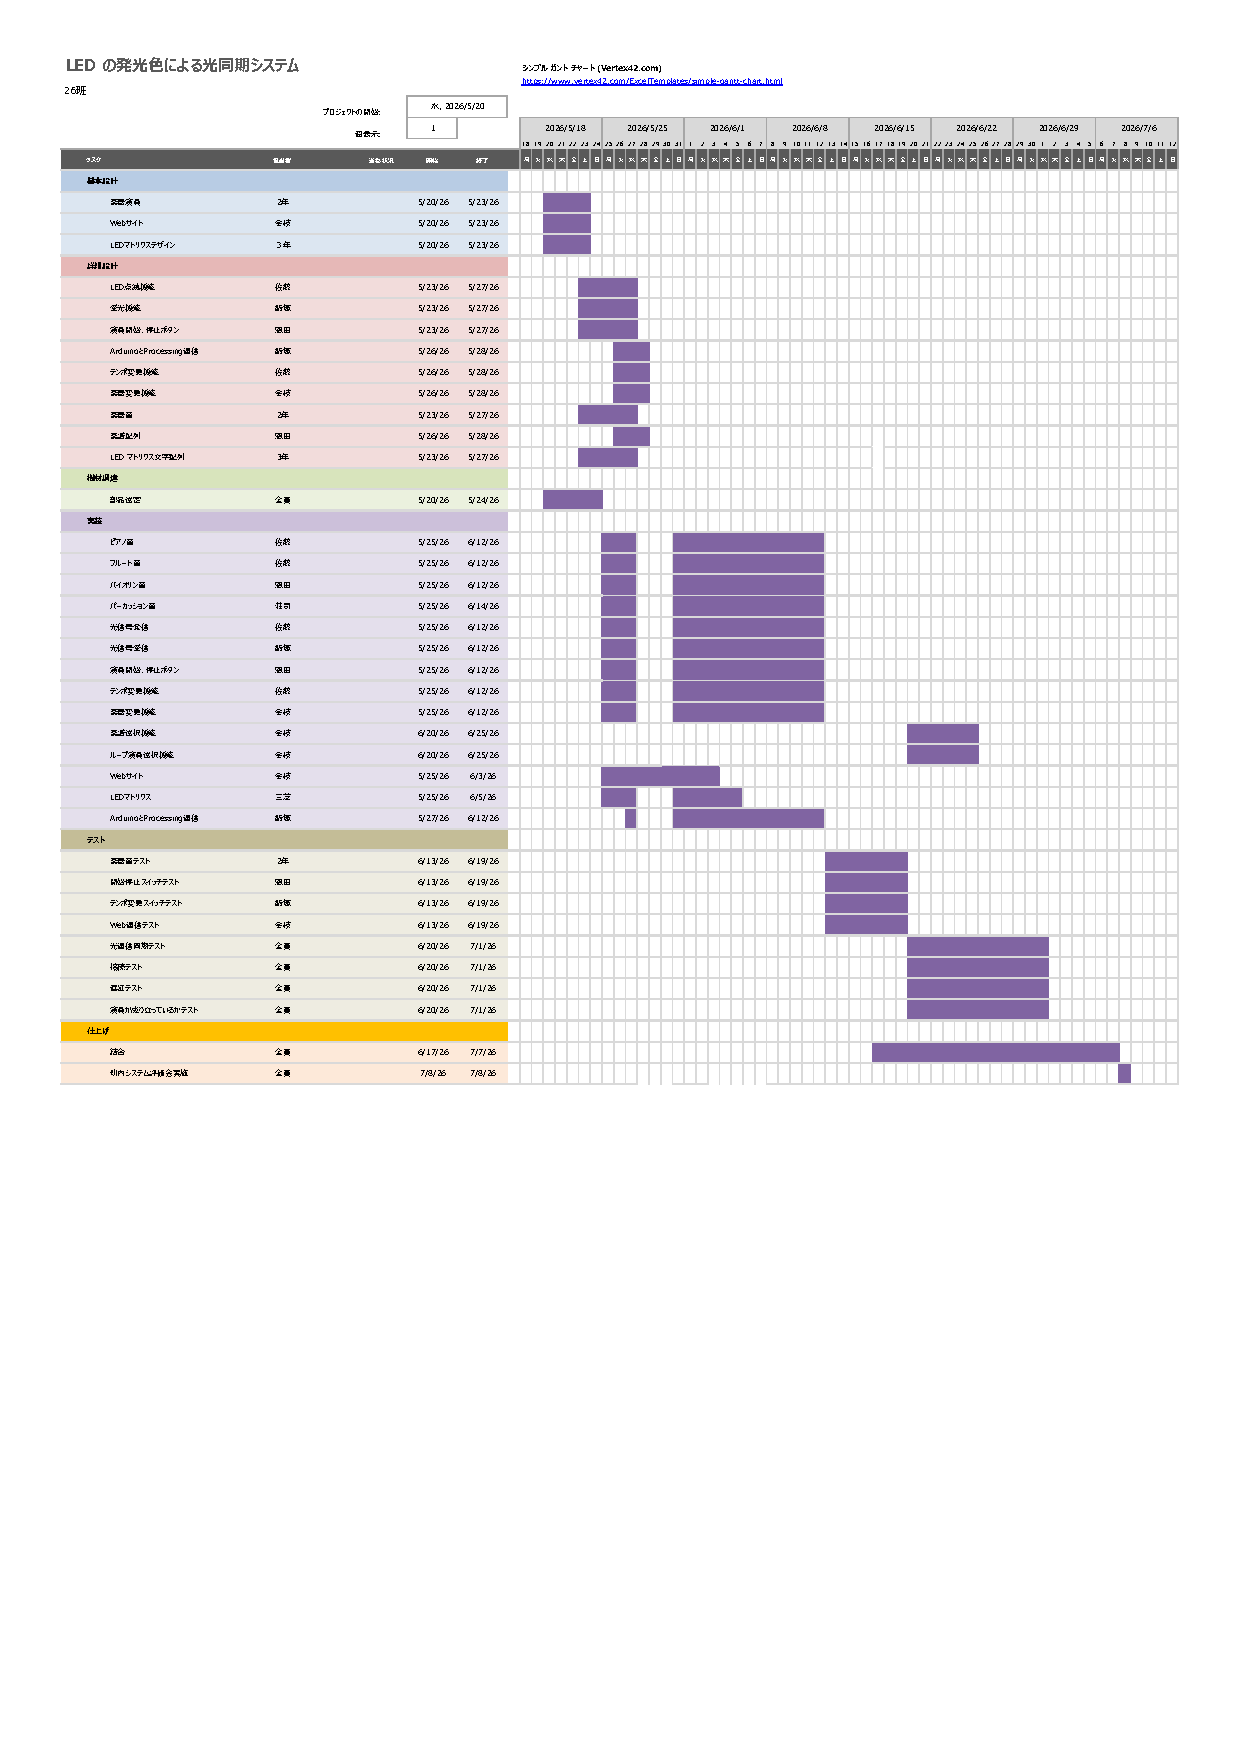
\includegraphics[width=14cm]{fig/gann7_1.pdf}
\caption{現在のガントチャート．}
\label{fig:ガントチャート変更後}
\end{figure}
\par

\clearpage

\section{技術成熟度レベルTRLの推移}
TRLの定義を以下の表\ref{TRL}に示す．
また，TRL定義に基づき，各作業の評価を行った．
その結果の推移を\ref{TRL推移}に示す．

\begin{table}[H]
\centering
   \caption{TRL定義}
   \label{TRL}
\begin{tabular}{|c|c|c|c|c|} \hline
1&概念レベル&アイディアや原理が確立されており，説明できるレベル\\ \hline
2& 基本動作レベル&単体で動作確認が可能なレベル\\ \hline
3&結合動作レベル&機能を結合し，実際の使用環境に近い環境で動作確認が可能なレベル\\ \hline
4&実運用レベル&実際の使用環境で安定的な稼働が確認できるレベル\\ \hline
 \end{tabular}
\end{table}

\begin{table}[H]
  \centering
   \caption{TRLの推移}
   \label{TRL推移}
  \renewcommand{\arraystretch}{1.2}
  \scalebox{0.68}{
    \begin{tabular}{|c|c|c|c|c|c|c|}
      \hline
        & 5週目 & 6,7週目 & 8週目 & 9週目 & 10週目 & 11週目 \\ \hline
      ピアノ音& 1 & 2 & 2 & 3 &4 & - \\\hline
      フルート音& 2& 2 & 2 & 3 & 4 & - \\\hline
      バイオリン音& 1 & 2 & 2 & 3 & 4 & - \\\hline
      パーカッション音& 1 & 2 & 2 & 3 & 4 & - \\\hline
      光信号送信& 1 & 2 & 3 & 3 & 4 & - \\\hline
      光信号受信& 1 & 2 & 3 & 3 & 4 & - \\\hline
      シリアル送信& 1 & 2 & 2 & 3 & 4 & - \\\hline
      シリアル受信& 1 & 2 & 2 & 3  & 4 & - \\\hline
      演奏開始/停止ボタン& 1 & 2 & 2 & 3 & 4  & - \\\hline
      テンポ変更機能& 1 & 2 & 2 & 3 & 4 & - \\\hline
      楽器変更機能& 1 & 2 & 2 & 3 & 4 & - \\\hline
      LEDマトリクス& 2 & 2 & 3 & 3 & 4 & - \\\hline
      カエルの歌楽譜配列& 2 & 2& 3 & 3 & 4 & - \\\hline
      webサイト& 2 & 3 & 3 & 4 & 4 & - \\\hline
      音色評価 & 1 & 2 & 3 & 3 & 4 & - \\\hline
    \end{tabular}
  }
\end{table}





\section{技術性能指標TPMの推移}
TPMの推移を表\ref{TPM推移}に示す．
本システムでは，通信同期性能および音色再現性能を定量的に評価するため，技術性能指標（TPM）を設定した．
各指標について，開発進行に伴う性能変化を継続的に記録する．

\begin{table}[H]
  \centering
   \caption{TPMの推移}
   \label{TPM推移}
  \renewcommand{\arraystretch}{1.2}
  \scalebox{0.68}{
    \begin{tabular}{|c|c|c|c|c|c|c|}
      \hline
       指標(単位) & 5週目 & 6,7週目 & 8週目 & 9週目 & 10週目 &11週目\\ \hline
      LED受信〜serial送信遅延 (ms)    & - & - & - & - & - & - \\ \hline
      serial送受信精度 (\%)           & - & 100 & 100 & 100 & 100 & - \\ \hline
      serial受信〜発音遅延 (ms)       & - & - & - & - & 0.1289115 & - \\ \hline
      同期ズレ (ms)                   & - & - & - & - & - & - \\ \hline
      パケット損失率(240) (\%)             & - & - & 0.0 & 0.0 & 99.88& - \\ \hline
      パケット損失率(180) (\%)             & - & - & 0.0 & 0.0 & 99.96 & - \\ \hline
      パケット損失率(120) (\%)             & - & - & 0.0 & 0.0 &  99.84& - \\ \hline
      パケット損失率(60) (\%)             & - & - & 0.0 & 0.0 & 100.00 & - \\ \hline
      パケット損失率(30) (\%)             & - & - & 0.0 & 0.0 & 100.00 & - \\ \hline


    \multicolumn{7}{|c|}{ピアノ} \\ \hline
      AT(立ち上がり時間)[ms]               & - & - & 39.8 & 39.8 & 39.8  & - \\ \hline
      SC(スペクトル重心)[\%]               & - & - & 17.1 & 17.1 & 17.1 & - \\ \hline
      DSV(スペクトル変動度)[\%]            & - & - & 11.84 & 11.84 &11.84  & - \\ \hline
      OER(奇遇倍音比)                     & - & - & 0.057 & 0.057 &0.057 & - \\ \hline
      \multicolumn{7}{|c|}{フルート} \\ \hline
      AT(立ち上がり時間)[ms]               & - & - & 29.9 & 29.9 & 29.9 & - \\ \hline
      SC(スペクトル重心)[\%]               & - & - & 16.7 & 16.7 & 16.7  & - \\ \hline
      DSV(スペクトル変動度)[\%]            & - & - & 4.76 & 4.76 & 4.76 & - \\ \hline
      OER(奇遇倍音比)                     & - & - & 0.041 & 0.041 & 0.041 & - \\ \hline
    \multicolumn{7}{|c|}{バイオリン} \\ \hline
      AT(立ち上がり時間)[ms]               & - & - & 39.8 & 39.8 & 39.8 & - \\ \hline
      SC(スペクトル重心)[\%]               & - & - & 12.2 & 12.2 & 12.2 & - \\ \hline
      DSV(スペクトル変動度)[\%]            & - & - & 11.67 & 11.67 & 11.67  & - \\ \hline
      OER(奇遇倍音比)                     & - & - & 0.097 & 0.097 & 0.097 & - \\ \hline
      \multicolumn{7}{|c|}{パーカッション} \\ \hline
      AT(立ち上がり時間)[ms]               & - & - & 0.0 & 0.0 & 0.0& - \\ \hline
      SC(スペクトル重心)[\%]               & - & - & 19.4 & 19.4 & 19.4 & - \\ \hline
      DSV(スペクトル変動度)[\%]            & - & - & 4.81 & 4.81 & 4.81 & - \\ \hline
      OER(奇遇倍音比)                     & - & - & 測定不可 & 測定不可 & 測定不可 & - \\ \hline
    \end{tabular}              
  }
\end{table}



\section{テストの実施日と結果}
テストは，システムの完成に基づき行うため，まだ未実施である．
システムテスト，単体テストは6月13日から6月19日，結合テストは6月10日から6月15日で行う予定である．
しかし，システムの完成に伴い行うことができるテストに関しては，可能な範囲で進めることにする．
それぞれテストの項目と，実施日，結果を以下の表\ref{システムテスト}，\ref{単体テスト}，\ref{結合テスト}に示す．


\begin{table}[H]
\centering
   \caption{システムテストの結果}
   \label{システムテスト}
\resizebox{\textwidth}{!}{
\begin{tabular}{|c|c|c|p{6cm}|c|c|c|} \hline
   ID&新/ 再&テスト項目 & テスト内容 & 実施日 & 結果 &コメント \\ \hline
   412&新&遅延テスト &ハイスピード撮影によりLED発光から発音までのフレーム数を計測し，遅延時間を算出する   & 6/24 & 88 ms & 正確な数値ではないが，目標の125 ms以内には収まっていた． \\\hline
   413&新&停止開始スイッチテスト &  Webサイトから開始・停止コマンドを送信し，演奏への反映を確認する& 6/24 & 合格 & 物理ボタンとwebどちらも開始，停止が可能 \\ \hline
   414&新&テンポ変更スイッチテスト & Webサイトからテンポ変更コマンドを送信し，演奏テンポへの反映を確認する & 6/24 & 合格 & ずれが生じる \\ \hline
   415&新&楽器変更スイッチテスト & Webサイトから楽器変更コマンドを送信し，演奏音色への反映を確認する& 6/24 & 合格 & 全楽器変更可能 \\ \hline
 \end{tabular}
}
\end{table}



\begin{table}[H]
\centering
   \caption{単体テストの結果}
   \label{単体テスト}
\begin{tabular}{|c|c|c|p{5cm}|c|c|p{4cm}|} \hline
  ID&新/ 再&テスト項目 & テスト内容 & 実施日 & 結果 &コメント \\ \hline
  411&新&ピアノ音 & 実際のピアノ音とシステム出力音のAT,SC,DSV,OERを算出し，音色再現精度を評価する& 6月17日& 合格 & - \\\hline
  411&新&フルート音&実際のフルート音とシステム出力音のAT,SC,DSV,OERを算出し，音色再現精度を評価する& 6月17日 & 合格 & - \\ \hline
  411&新&バイオリン音&  実際のバイオリン音とシステム出力音ののAT,SC,DSV,OERを算出し，音色再現精度を評価する& 6月17日 & 合格 & - \\ \hline
  411&新& パーカッション音&実際のパーカッション音とシステム出力音のAT,SC,DSVを算出し，音色再現精度を評価する & 6月17日 &合格 & OERは，スネアの音構成により，倍音構造が検出できないためOERは評価しない \\ \hline
 \end{tabular}
\end{table}
アンケートで実際の可聴音の評価も同時に行っている．



\begin{table}[H]
\centering
   \caption{結合テストの結果}
   \label{結合テスト}
\begin{tabular}{|c|c|c|p{5cm}|c|c|p{4cm}|} \hline
   ID&新/ 再&テスト項目 & テスト内容 & 実施日 & 結果 &コメント \\ \hline
   421&-&光通信同期テスト &光同期通信を一定回数実施し，送受信ログを比較してパケット損失率（IPLR）を算出する  & 7/1 & 合格 & 複数のテンポで計測を行ったがいずれも99\%を超える結果となった． \\ \hline
   422&新&接続テスト &  複数の演奏者PCを接続し，正常に通信が確立されることを確認する& 6/24 & 合格 & - \\\hline
   423&-&遅延テスト & ハイスピード撮影により全体演奏者PC間の発音フレームのズレを計測し，同期遅延を算出する & - & - & - \\ \hline
 \end{tabular}
\end{table}
% 同じ音で同じタイミング: 楽器間の同期ずれ(同じで2つ鳴らして両者間の音のズレが40ms以内)
% 同じ音でやらないと立ち上がりの音の違いで差が出てしまう．
% 全体の演奏ズレ: 全部一気に撮って全体の差が40 ms以内



\section{その他}
%• [連絡事項・懸念点など]
特になし．



\end{document} 
